\documentclass[12pt,Bold,letterpaper,TexShade]{mcgilletdclass}
\usepackage{graphicx}
\usepackage{geometry}
\usepackage{texshade}
%\usepackage{setspace}
%\singlespacing
%\onehalfspacing
%\usepackage{tex4ht}
%\usepackage{amsmath}
%%%%%%%%%%%%%%%%%%%%%%%%%%%%%%%%%%%%%%%%%%%%%%%%%%%%%
%% Have you configured your TeX system for proper  %%
%% page alignment? See the McGillETD documentation %%
%% for two methods that can be used to control     %%
%% page alignment. One method is demonstrated      %%
%% below. See documentation and the ufalign.tex    %%
%% file for instructions on how to adjust these    %%
%% parameters.                                     %%
\addtolength{\hoffset}{0pt}                        %%
\addtolength{\voffset}{0pt}                        %%
%%                                                 %%
%%%%%%%%%%%%%%%%%%%%%%%%%%%%%%%%%%%%%%%%%%%%%%%%%%%%%
%%       Define student-specific info
\SetTitle{\huge{Combining Genetic Algorithms with Physical Simulation}}%
\SetAuthor{Guillaume Labranche}%
\SetDegreeType{COMP-521 Final Project}%
\SetDepartment{School of Computer Science}%
\SetUniversity{McGill University}%
\SetUniversityAddr{Montreal, Quebec}%
\SetThesisDate{2015-04-14}%
%\SetRequirements{ \\}%
%\SetCopyright{Copyright Guillaume Labranche}%

%\makeindex[keylist]
%\makeindex[abbr]

%% Input any special commands below
%\newcommand{\Kron}[1]{\ensuremath{\delta_{K}\left(#1\right)}}
\listfiles%
\renewcommand{\thesection}{\arabic{section}}
%\setcounter{sectocdepth}{1}
%\dou­blespac­ing
\begin{document}

\maketitle%

\setcounter{secnumdepth}{4}
\setcounter{tocdepth}{4}
\begin{romanPagenumber}{2}%

\TOCHeading{\MakeUppercase{Table of Contents}}%
%\LOTHeading{\MakeUppercase{List of Tables}}%
%\LOFHeading{\MakeUppercase{List of Figures}}%
\tableofcontents %

\end{romanPagenumber}

%\setcounter{secnumdepth}{1}
%\setcounter{section}{0}

%\mainmatter %
\GoDouble

 
\section{Introduction}
%state the main objectives of the project, briefly describe the methodology, and summarize the results. For those working in groups, separately and clearly identify what was done by each person in terms of the project content, and also the report itself.
The main objectives were to make a computer find the best configuration for a car over an accidented terrain without prior knowledge of design strategies. In order to achieve such a result, I used evolutionary algorithms based on genetics to find the best configuration by trial and error. ~\cite{Geijtenbeek2013}

\section{Background}
%give background on the problems you are addressing. This should include at least 2 technical references (by which I mean academic books/papers or detailed industry explications, and not just websites/blogposts).
Evolutionary algorithms have many advantages: ~\cite{miller1995genetic}
\begin{itemize}
\item They are modelled after nature -- and nature is ahead of us in terms of engineering.
\item It allows for entertaining visualizations. Seeing the algorithm do its work, and vehicles improve as it works through the generations is nice.
\item Not much engineering of our own is needed. We just have to program the algorithm properly, and it will work through any challenge thrown at it. ~\cite{MIM}
\end{itemize}

A nice property is their modularity, similar to compilers that are divided into distinct phases.

\section{Methodology}

\subsection{Fitness Measurement}

Measuring the fitness of an individual was made through simulating a physics-based environment in which certain capabilities would need to be optimized in order to success. I decided to represent my individuals as vehicles with an arbitrary shape and placement of wheels. The goal for them was to travel over a rough terrain (to add complexity, since simply a vehicle going over flat land is easy to create). The fitness measure was then how far they were able to travel before stalling.

\subsubsection{Vehicles}

The vehicles consist of a set of 8 vertices all randomly distributed around a center point. This defined the vehicle's chassis (frame) on which to attach wheels. Each vertex has a probability (20\% in practice) of having a wheel at its tip. The vehicle's weight is also calculated from the triangles making up its \verb|Mesh|. It is then set as a property of the \verb|RigidBody2D| to create more realistic simulations (heavy vehicles have a hard time going uphill but are more stable). Each wheel also has a weight dependent on its radius ($\pi r^2$).

\subsubsection{Terrain}

I initially tried to use a well-made Unity plug-in but it had not been updated in a while and Unity itself had upgraded two versions since. I therefore wrote my own simple implementation. The process is quite simple: each new segment is based on the previous, and subject to some constraints. The constraints are namely:

\begin{itemize}
\item An absolute minimum/maximum slope throughout all the terrain.
\item A maximum change of angle between connected segments.
\item An easiness factor that affects the first 40 segments, where the above two constraints are multiplied by $i/40$ where $i$ is the index of the segment.
\end{itemize}

The third factor makes the terrain rather flat at the beginning, so that the evolutionary algorithms can optimize for basic movement before getting into more challenging terrain. Otherwise it would be very possible to have a very rough edge right at the start, and our first generation of vehicles would not be able to get over it. We would then not get any information out of this since everybody got a close fitness score.

The new segment's length is fixed for all. Its angle is then chosen randomly through a uniform distribution that is the maximum window satisfying the previously-mentioned constraints. It leads to a terrain that is quite natural-looking.

\subsection{Evolution}
% https://en.wikipedia.org/wiki/Genetic_operator

\subsubsection{Selection}

This is the part that deals with selecting the best individuals in order to improve the gene pool. In essence, this algorithm uses the fitness factors computed with our physical simulation to take a subset of the population with a higher score average than that of the entire population. It then uses the selected set of individuals for "mating" or "reproducing". There are many ways of doing this, such as always simply selecting the best individuals, or choosing randomly a fixed number of individuals with a weighted probability distribution using the fitness scores. I chose to implement the technique called "tournament" ~\cite{miller1995genetic} which goes like this: we select $k$ individuals from the population, and only keep the highest individual (some versions keep the top $t$ highest, where $t<=k$). We proceed until there are less than $k$ individuals in the population. This leads to $n/k$ individuals (where $n$ is the size of the gene pool) to be passed onto the crossover phase. An advantage of this technique is that there is a significant amount of randomness, which assures that we do not over over-select some properties at the beginning and end up in a local maxima.

\subsubsection{Crossover}

The crossover phase deals with mating two individuals and to create two offspring who keep some properties of their parents. Basically, this takes care of keeping the good traits that the top-scoring selected individuals have, and even improve on it. Again, many techniques have been developed for this. The main ones treat the chromosome (set of values that define an individual's traits) as a sequence of numeric values and split it in different ways, such that some parts are given to the first children and other parts to the other. In my implementation, I used the two-point crossover technique, which yielded good results right away. In my particular physical model, this proved to be efficient since the vertices defining the chassis of the vehicle are stored in counter-clockwise order. Therefore, if an individual has some part of his body that benefits him greatly (such as a concave section between two wheels), it is more likely to be part of a single segment and to be untouched and reproduced in one children.

\subsubsection{Mutation}

Mutation is the last step in the process of evolution. It deals with introducing random changes throughout the genome in order to provoke improvements (or handicaps) within all individuals. If it was not present, the algorithm would certainly optimize the initial configuration but the best performing individuals might not be exposed to unplanned changes which could benefit their performance. In the real evolution of species, it is the result of drastic changes in populations. In practice, this is done by setting a mutation probability and for every chromosome, assign a new random value to it if a random variable is under the probability.

\section{Results}
%describe the experimental context/strategy, and give numerical (tables and/or graphs) data summarizing your results. Include discussion of anomalies, trends, and any other interesting observations you can make on the data.

As a result of this project, vehicles are found to travel through the accidented terrain within a few generations. As we can see in Figure \ref{fig:plots}, the average increases steadily.

\begin{figure}[p]
    \centering
    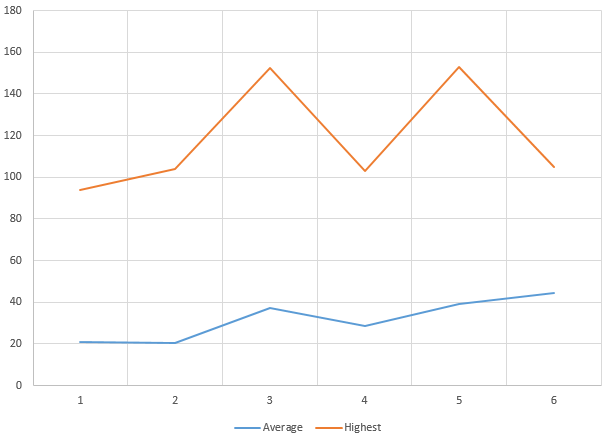
\includegraphics{plot1.png}
    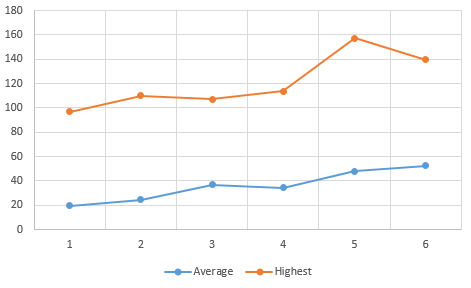
\includegraphics{plot2.png}
    \caption{Scores per generation}
    \label{fig:plots}
\end{figure}
%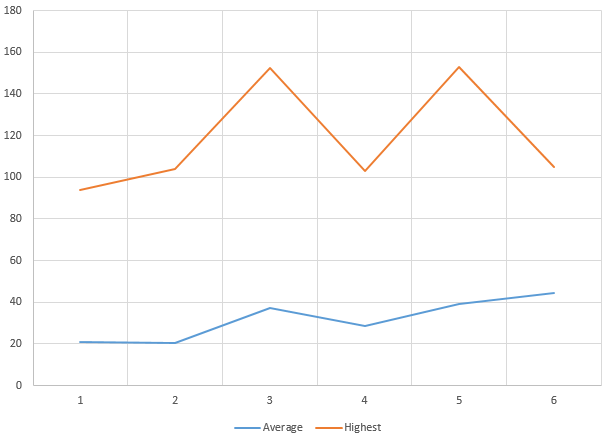
\includegraphics{plot1.png}

\section{Conclusion}

In conclusion we see that evolutionary algorithms are both powerful and entertaining. They can adapt to a wide range of problems and require less implementation code than the custom algorithms adapted to the specific case.

We could extend to other forms of physical simulation. We could also add user interaction such a designing their own cars to try to compete against the algorithms.

%\SetAppendixName{References}%
%\SetAppendixText{List of references}
%\ETDAppendix{References}{Here is the text of an Appendix.}%}%
%fjklsdafjklsdafjkldasjfkldjaskl
%\end{\ETDAppendix}%
\bibHeading{References}
\bibliography{report}
\bibliographystyle{plain}

\end{document}


 






